\section{Approach}

We first present the preliminaries on stress test operators to create stress 
test cases for measuring model robustness,
%We first describe stress test operators for evaluating robustness in models. 
%, and adopt a subset of them as proxy test for short circuits. 
then propose two novel operations to augment training data to 
%reverse the short circuit problem and 
enhance the model robustness.

\subsection{Preliminaries}
 \label{sec:stressop}
%Short circuit behavior can be considered as a specific type of model fragility. 
The typical approach for detecting and evaluating model fragility is to construct out-of-distribution stress tests in addition to the original in-distribution test set and observe model performance on these stress tests.

In this paper, we consider the operators for constructing stress test listed in \tabref{table:proxyop}. 
The perators were mentioned in previous literature\cite{checklist2020acl}. 
%others are proposed here~(marked with *). 
Each operator creates a stress test instance corresponding to a specific MCQ by keeping the right choice and 
generating a new \textbf{wrong} choice. 
%The new wrong choice can be generated \KZ{either from the right choice 
%or the wrong choice of the original MCQ.}
%c) right choice of another randomly 
%sampled MCQ. 

\begin{table}[th]
        \centering
        \scriptsize
        \begin{tabular}{l|l}
                \toprule
                \textbf{Oper.} &\textbf{Description and Example}\\
                \hline
                \multirow{3}{*}{Neg+} & Add negation (r$\rightarrow$w) \\
                & Input: \textit{They called the police to come to my house. \checksymbol} \\
                & Output: \textit{They {\textbf{{didn't}}}  called the police to come to my house. \crosssymbol} \\
                \hline
                \multirow{3}{*}{Neg-} &Remove negation (r$\rightarrow$w) \\
                & Input: \textit{Ben {\textbf{never}} starts working out. \checksymbol} \\
                & Output: \textit{Ben starts working out. \crosssymbol}\\
                \hline

                \multirow{3}{*}{NER} &Randomly replace person names (r$\rightarrow$w)\\
                 & Input: \textit{A big wave knocked {\textbf{ Mary}} down . \checksymbol} \\
                & Output: \textit{A big wave knocked {\textbf{ Kia}} down . \crosssymbol} \\
                \hline
                \multirow{3}{*}{PR} & Switch pronoun by gender or quantity (r$\rightarrow$w)\\
        &Input: \textit{{\textbf{ She}} had a great time .\checksymbol} \\
        &Output: \textit{{\textbf{ He}} had a great time . \crosssymbol} \\
                \hline
                \multirow{3}{*}{PI} &Instantiate pronoun by randome person (r$\rightarrow$w) \\
        &Input: \textit{{\textbf{ They}} gave Tom a new latte with less ice . \checksymbol}\\
        &Output: \textit{{\textbf{ Nathanael}} gave Tom a new latte with less ice . \crosssymbol}\\
        \hline
        \multirow{3}{*}{Voice} &Swap subject and object (r$\rightarrow$w) \\
        & Input: \textit{{\textbf{Kara}} asked {\textbf{the neighbors}}  not to litter in their yard . \checksymbol} \\
        & Output: \textit{{\textbf{the neighbors}} asked  {\textbf{Kara}}  not to litter in their yard . \crosssymbol}\\
%               %\hline
                %\multirow{3}{*}{Adv*} &Add adverbs for emphasis (w$\rightarrow$w)\\
                %&Input: \textit{The ocean was as calm as a bathtub .\crosssymbol} \\
                %&Output: \textit{{\textbf{ In fact}} the ocean was as calm as a bathtub .\crosssymbol} \\
  %:ew              \hline
              % \multirow{3}{*}{CO*} & Crossover: Swap the true choices between two questions (r$\rightarrow$w)\\ 
        %&Input: \textit{\textbf{olive}Josh got sick . \checksymbol} \\
        %&Output: \textit{\textbf{olive}{She had a great time .\crosssymbol}}  \\
%\hline
 %               \multirow{3}{*}{Syn} &Replace adj/adv with synonym (w$\rightarrow$w) \\
 %               &Input: \textit{Dawn felt {\textbf{ happy}} about getting away with it . \crosssymbol} \\
 %               &Output: \textit{Dawn felt {\textbf{ glad}} about getting away with it . \crosssymbol} \\
              % \multirow{3}{*}{MT*} & Mutate: Swap two consecutive words (r/w$\rightarrow$w) \\
        %       & Input: \textit{Deb said yes {\textbf{olive} to} {\textbf{olive} Tim} 's marriage proposal. \crosssymbol} \\
        %       & Output: \textit{Deb said yes {\textbf{olive} Tim} {\textbf{olive} to} 's marriage proposal .\crosssymbol} \\
        %       & Input: \textit{Josh {\textbf{olive}got sick}. \checksymbol} \\
        %       & Output: \textit{Josh {\textbf{olive} sick got}. \crosssymbol} \\
          %     \hline

                \bottomrule
        \end{tabular}
        \caption{Stress test operators considered in this paper. 
The first line in each cell describes the operation, the remaining lines in
the cell give examples of how the operators work.
r$\rightarrow$w indicates the operator turns a right choice into a wrong choice.}
%while
%w$\rightarrow$w indicates the operator turns a wrong choice into another wrong choice.}
        \label{table:proxyop}
\end{table}

All operators listed in \tabref{table:proxyop} 
%\textit{Neg+}, \textit{Neg-}, \textit{NER}, \textit{PR}, 
%\textit{PI}, and \textit{Voice} 
convert an original \textbf{right} choice into a new \textbf{wrong} choice 
that is linguistically similar to the original right choice. 
The resultant stress test cases are not only able to 
evaluate the general model robustness, but also 
whether models are exploiting spurious features in the choices alone 
rather than considering the connection between the premise and choices. 
%The remaining two operators \textit{Adv} and \textit{Syn} 
%generate a new wrong choice that is semantically similar to 
%the original wrong choice.
%For \textit{Adv}, we randomly insert an adverb from the list (``in fact'', ``actually'',
%``indeed'') as the prefix to the wrong choices.
%The adverb operator is not used for training but for testing.
% The purpose of these two operators is to trick the models into selecting the wrong choices
% without looking at the premises. 
%\KZ{Why??}
%thereby making them not suitable for testing short-circuiting. 

%\subsection{Proxy Test for Short Circuit}
%\label{sec:proxytest}
%\subsubsection*{Attention Score Analysis}
%We propose a black-box framework to test short circuits in models. 
%As In a black-box testing, 
%if a model correctly answers an MCQ, we create a new MCQ from
%the old one by keeping the right choice of the old MCQ and 
%generating a new wrong choice. The new wrong choice is generated by operations upon either the right choice of the old MCQ or the right choice of another randomly sampled MCQ.

%These operations can create additional questions from
%original ones to serve as stress test. We will discuss
%the suitability of these two operations for creating
%short-circuit tests. 
%\cut{%%%%%%%%%%%%%%%%%%%%
%\subsubsection{White-box Attention Weights~(AW)}
%\KZ{Here we first talk about human testing by visualizastion,
%then talk about how to automatic it thru code.}

%show human annotation results of bert, roberta, xlnet.
%One intuitive way to detect if an attention-based model is 
%exploiting short circuits is to visualize its attention map. 
%Given a well-trained model and a correctly answered MCQ  in the 
%form of \textit{[CLS] premise [SEP] choice [SEP]}, 
%where \textit{[CLS]} and \textit{[SEP]} are model-dependent 
%delimiters and \textit{choice} refers to the right choice, 
%we first tokenize the input, feed the token sequence into the model, 
%and extract the attention map of all attention heads from the 
%last encoder layer.
%
%The attention maps are visualized through off-the-shelf tool~\cite{vig-2019-multiscale}
%into user-friendly demo as shown in \figref{fig:att-goodex}. 
%Human annotators are then asked to determine whether there exists 
%strong attention connections from the right choice to the premise. 
%We consider the MCQ is solved without short-circuiting only if 
%over half of the annotators label it as having strong attention 
%connections. 
%
%Though accurate, such manual annotation is cost-prohibitive to be 
%scaled to larger tests. To remedy this issue, we propose 
%a rule-based procedure to automatically detect the short circuit 
%behavior of a model on MCQ. Specifically, we aggregate the 
%attention maps into one individual map by max-pooling over all 
%attention heads. Then we check if there exists at least one 
%attention score between token in the choice and token in the premise 
%higher than threshold $t_1$ or at least two higher than threshold 
%$t_2$, excluding special tokens like comma and period. 
%We consider that the model not short-circuiting on this MCQ if 
%neither of the two conditions is met. In practice, the 
%threshold $t_1$ and $t_2$ are tuned so as to maximally simulate 
%human annotation. 
%Human annotators are 
%asked to determine whether there exists a strong visual correlation
%between the correct choice and the premise. We consider the model not
%short-circuiting only if more than half of the human annotators
%confirm a strong correlation. 
%$t_1$ is greater than$t_2$. The pseudo-code is shown in Algorithm \ref{AW}.
%
%%show the automatic procedure for testing reasoning short circuit.
%\begin{algorithm}
%\small
%       \caption{Attention Weight Thresholding}
%       \label{AW}
%\hspace*{0.02in} {\bf Input:} 
%premise $P$, correct choice $C$, model $M$,  threshold $t_1$ and $t_2$. \\
%\hspace*{0.02in} {\bf Output:}
%binary 0/1 label $L$.
%       \begin{algorithmic}[1]
%               \State initialize counters $c_1$ and $c_2$ to 0.
%               \State tokenize the formatted input as sequence of tokens $S$.
%               \State feed $S$ into $M$ and extract the last layer's attention maps $Attn_{all}$.
%               \State aggregate $Attn_{all}$ into $Attn_{max}$ by max-pooling over all attention heads.
%               \For{$w_1$ in $C$}
%               \For{$w_2$ in $P$}
%               \If{$Attn_{max}(w_1, w_2)> t_1$}
%                               $c_1$ += 1
%               \EndIf
%               \If{$Attn_{max}(w_1, w_2) > t_2$}
%                               $c_2$ += 1
%               \EndIf
%               \EndFor
%               \EndFor
%               \State output 1 if $c_1>0$ or $c_2\geq 2$ and 0 otherwise.
%       \end{algorithmic}
%\end{algorithm}
%
%
%\subsubsection*{Black-box Choice Operator}
%\label{sec:proxy}
%}%%%%%%%%%%%%%%%%%%end of cut %%%%%%%%%%
%\subsubsection*{Crossover Blackbox Testing}
%The attention-based testing method is more accurate 
%but it is restricted to model family with inherent attention mechanism. 
%The attention-based testing methods can detect short circuits within the encoder 
%directly, but strictly speaking, they are not detecting the
%short circuits in the end-to-end MCQ model, which additionally includes a linear layer
%above the attention-based pretrained language model. 
%In addition, they are restricted to only a family of models 
%with inherent attention mechanism, which limits their use.
%%As an alternative, we propose the crossover black-box testing inspired by molecular biology.
%
%%When developing a cross-model testing, one of the most frustrating challenges 
%%is the difficulty in testing models cross different structures. 
%%In addition, the attention-based testing method is more accurate 
%%but it is restricted to model family with inherent attention mechanism.
%What is more desirable is an automatic end-to-end black-box test
%which is  model independent. 

%By observing the model's response to the new MCQ, 
%we can infer whether the model short circuits on the right choice of the old
%MCQ \footnote{A model may short circuit either in the right choice or
%in the wrong choice, the latter of which corresponds to the ``exclusion
%principle.'' Our proxy tests are designed to identify the first type, 
%because a) by observation the second type seldom happens; and b) 
%to properly treat the second type, one has to synthesize
%a valid premise for the wrong choice, which is very difficult.}. 
%If the model still picks up the right choice, then we consider
%it passes the test, and did not short-circuit on the
%old MCQ. The question now is how to construct
%the new wrong choice by implementing some of the stress test operations 
%in different ways.

%Inspired by boundary testing in software engineering, 
%we can classify the stress test operators introduced in \secref{sec:stressop} into three
%equivalent classes (delimited by the thick lines in \tabref{table:proxyop}), 
%depending on the nature of
%the \textit{wrong} choice it constructs:
%\begin{enumerate}
%\item The syntax and semantics are correct, and 
%the \textit{wrong} choice appears similar to the \textit{right}
%choice.
%\item The syntax and semantics are correct, and 
%the \textit{wrong} choice appears distinct from 
%the \textit{right} choice. 
%\item Either syntax or semantics is incorrect.
%\end{enumerate}

%We do not adopt Adv~\cite{wsp2020acl} and Syn~\cite{checklist2020acl,wsp2020acl} in the second class in short circuit testing because they operate on wrong choices. The last class is also not suitable for testing
%short circuits, because the model may answer the proxy question
%correctly by eliminating the wrong choice due to
%the errors in it, not by looking at the premise. For the above reasons, we only consider perturbations on 
%negation~\cite{checklist2020acl}, NER~\cite{checklist2020acl}, 
%and pronouns in the first class and 
%crossover in the second class as proxy tests for short circuit
%in this paper.
%\begin{example}\label{ex:crossover}
%       \begin{description}
%               \item[Context:] The student knew the answer to the question.
%               \item[Choice 1:] He raised his hand . \Checkmark
%               \item[Original Choice 2:] He goofed off .\XSolidBrush
%               \item[Crossed Choice 2:] Dust got into his eyes.\XSolidBrush
%       \end{description}
%\end{example}

%Compared with all other operations in class 1 and 2, 
%crossover gives a proxy question that is most different from the original one,
%but easier from human's perspective, because now the two choices maybe
%quite unrelated. If the proxy question is not done correctly by the model, 
%it's more indicative of a short circuit. So potentially, crossover
%is a better short circuit test than others. 


%Another advantage of crossover is that we can generate many wrong choices 
%for an original question at a low cost, thus we can test each original question
%more thoroughly. Whereas most other operations cannot produce 
%variants of the original choice in large quantity. 
%%The test cases for the third part is easy to construct, like mutation and voice~\cite{wsp2020acl}. 
%%However, this type of testing is not sufficient to assess 
%whether the model has reasoning capabilities, 
%because solving these new cases does not require understanding of the previous premise. 
%We can't say for sure which of the reasons for the failure of 
%a specific case, 
%but it still reflects whether the model is robust or not. 

\subsection{Improving Model Robustness by Data Augmentation}
\label{sec:aug}
If a model is shown to be fragile by the stress tests, 
its performance may decline, especially when applied to out-of-distribution test data.
%We make an assumption that these models are 
%limited by dataset and learned short circuits to make decision. 
To make models more robust, one natural thought is to generate more data to encourage models to focus on the 
relation between the premise and choices.
Intuitively, all the operators that can generate stress tests
can be used to create more training data.
But in reality, most of these operators are not scalable and 
cannot generate enough data for training, e.g., \textit{NER} requires the presence of named entities in the choices.
Meanwhile, these stress test operators are fine-grained operations on specific features, 
and it's hard to enumerate all the possible features for training, not to mention 
their combinations. 

To overcome the above issues,
we propose two genetically inspired operators, 
namely \textit{crossover} and \textit{mutation}, 
which are more scalable and generally applicable for data augmentation.
These two operators are  
not only simple but also not limited to the fine-grained features. 

\begin{figure}[htbp]
        \centering
        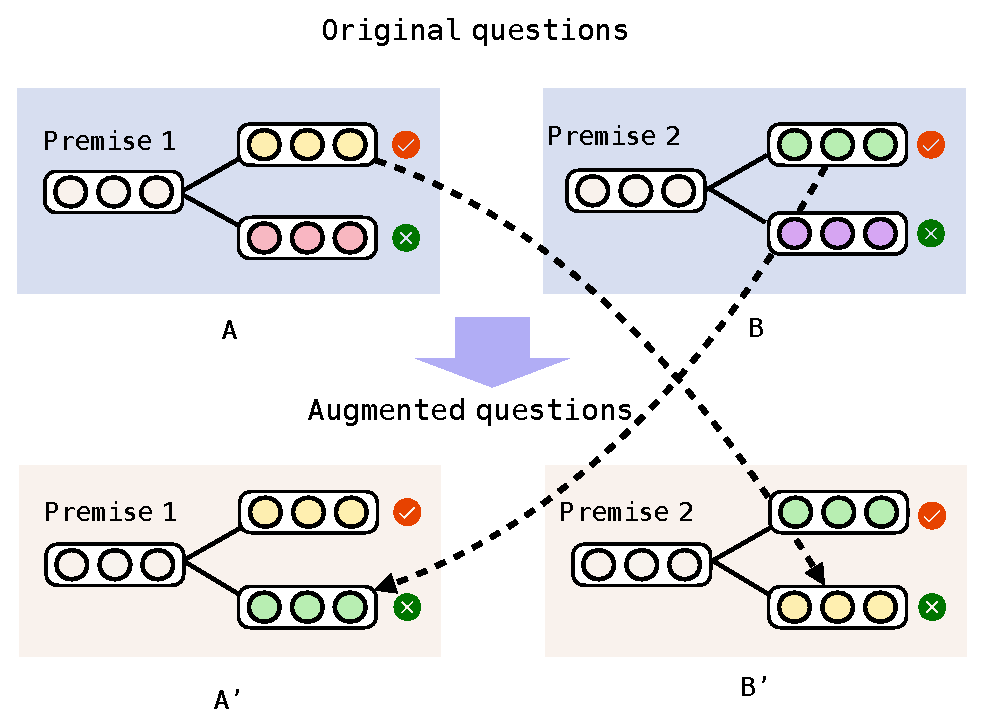
\includegraphics[width=0.8\columnwidth]{figure/cross.eps}
        \caption{Crossover: the right choice of both questions
                are used to replace the wrong choices of these questions to create
                two new questions. Circles symbolizes tokens in the sentences.}
        \label{fig:cross}
\end{figure}
\begin{figure}[th]
        \centering
        \includegraphics[width=\columnwidth]{figure/revised_mutation.eps}
        \caption{Mutation: the right choice of a question
                is used to replace the wrong choices of this question to create
                new questions. Circles symbolizes tokens.}
        \label{fig:mutation}
\end{figure}
%\KZ{Above table doesn't have mutation. 
%Move mutation to after crossover. introduce crossover first.
%You commented out a lot of stuff above about crossover and mutation.
%Why can't u reuse some of that stuff?}
\textit{Crossover} is illustrated in \figref{fig:cross}. It operates 
on two randomly selected MCQs.
We substitute the wrong choice of one MCQ with the right choice from 
the other MCQ to generate a new MCQ. The substituted choice is 
almost certainly wrong in the new MCQ. 
For example, the green choice in $B$ is the right choice, 
but wrong for the new question ${A}'$. 
We only consider swapping the right choices between 
two questions rather than wrong ones. 
This is because if the model was short-circuiting,
then it is likely to rely on some spurious features correlated with the true
label in the right choices. 
By substituting these right choices into another question to make them wrong, 
this operation can disrupt such correlations.
Hence, to tell if one choice is better than the other, 
the model is encouraged to consider the premise. 




%Besides the quantity, crossover is a good option for data augmentation,

%If we swapped the wrong choices, we could 
%still produce two legitimate new questions. But these new questions can't
%test short circuit, because: a) if a model
%short-circuits on the right choice of question B (as in \figref{fig:cross}), 
%swapping the wrong choice of B into question A doesn't make A' a good test, 
%since the model is not sensitive to wrong choice; 
%b) if a model short-circuits on the wrong choice of
%question B, swapping the wrong choice of B into A will make A' 
%easier to solve by the model, so it will 
%still pick the right choice and pass the test.

%We can also teach them to discover semantic and syntax problems with the advantage of the choice question format. 
%\KZ{Crossover not only can be used to test for
%short circuit, it can also be used to improve the model
%robustness. How to?}
%Both methods actually have the potential to teach the model 
%to consider the previous premise. First of all,  crossover is a replacement for the ``True'' choices, 
%models can not get the correct answer from the choices alone. 
%\KZ{The crossver operation inspired us to try mutation.}
\textit{Mutation} is illustrated in \figref{fig:mutation}. 
\textit{Mutation} operation swaps two consecutive words either in 
the right choice or wrong choice of 
the original MCQ, each with 50\% probability, to make a new wrong choice.
%Compared to crossover,
The \textit{mutation} operator should not be confused with the random token
swapping (RS) operator~\cite{artetxe2017unsupervised,lample2017unsupervised}.
RS seeks to perturb a choice in the question without changing its label,
whereas mutating the right choice (\textit{mutation}) converts it to a wrong choice because the 
perturbed choice is ``less right'' than the original one.
Mutating the wrong choice has the similar effect as RS.
%lots of work mentioned randomly swapping tokens (mutation)
%(Artetxe et al., 2018; Lample et al., 2018; Wei and Zou, 2019; Miao et al., 2020),
%The purpose of RS is to improve models' fault tolerance by perturbing
%the sentence without changing its meaning;
%the purpose of our mutation is to encourage the models to look into the
%premise (thus avoid short-circuits).
%Consequently, the way we construct the data is also different. 
Intuitively, mutation has the potential to improve model robustness:
it not only encourages the model to look into the premise due to its
two very similar choices (see the two choices of A1 in \figref{fig:mutation}), 
but also makes the model more sensitive to the differences in word orders 
and enhances the model's pre-existing grammatical knowledge (see the two choices in
A2). 
%Discuss the pros and cons of the two.
%Explain why mutation may not be a good choice for detecting
%short-circuit.

